\documentclass{beamer}
\usepackage[utf8]{inputenc}
\usepackage[english,russian]{babel}
\usepackage{hyperref}
\usepackage{xcolor}
\usepackage{graphicx}

\usetheme{Boadilla}
\usecolortheme{seahorse}
\setbeamercovered{transparent}% Allow for shaded (transparent) covered items

\AtBeginSection[]
{
  \begin{frame}
    \frametitle{Содержание}
    \tableofcontents[currentsection]
  \end{frame}
}

\begin{document}

\title[]{Многоагентные системы}
\author{Н.\,Д.~Кудасов}
\institute{МГУ им. Ломоносова}
\date{Москва, 2013}

\begin{frame}
\addtocounter{framenumber}{-1}
\maketitle
\end{frame}

\section{Концепция агента}

\begin{frame}
  \frametitle{Что такое агент?}
  \begin{exampleblock}{}
    {\large ``Агент~--- это инкапсулированная вычислительная система,
    помещенная в некоторую среду и способная автономно выполнять действия
    в этой среде для достижения поставленных целей.''}
    \vskip5mm
    \hspace*\fill{\small--- Wooldridge and Jennings \cite{Wooldridge1995}}
  \end{exampleblock}

  \begin{exampleblock}{}
    {\large ``Агент~--- это вычислительная система, автономно действующая от лица других
    сущностей, выполняющая действия реактивно и/или с определенной целью и в некоторой
    степени использующая свойства обучаемости, кооперативности и мобильности.''}
    \vskip5mm
    \hspace*\fill{\small--- Shaw Green et al. \cite{Green1997}}
  \end{exampleblock}
\end{frame}

\begin{frame}
  \frametitle{Общее понятие агента}
  В самом общем случае агент обладает следующими свойствами:

  \begin{itemize}
    \item<1-> {\it реактивность}: способность агента воспринимать окружающее и влиять на него;
    \item<2-> {\it целеустремленность}: агент должен действовать в заложенными в него целями;
    \item<3-> {\it социальная активность}: агент должен взаимодействовать с другими агентами и/или людьми;
    \item<4-> {\it автономность}: агент действует без непосредственного вмешательства человека и обладает
      определенным контролем на своими действиями и внутренним состоянием.
  \end{itemize}
\end{frame}

\begin{frame}
  \frametitle{Ментальные характеристики}
  Распространено использование ментальных характеристик:

  \begin{itemize}
    \item знания,
    \item убеждения,
    \item намерения,
    \item обязательства и т.п.
  \end{itemize}

  Иногда агенты наделяются {\it эмоциями}.
\end{frame}

\begin{frame}
  \frametitle{Прочие свойства}
  Часто также используются следующие свойства агентов:

  \begin{itemize}
    \item<1-> {\it мобильность}: способность агентов перемещаться \\ (физически или в сети);
    \item<2-> {\it правдивость}: предположение, что агент не может намеренно фальсифицировать передаваемую (другим агентам, человеку) информацию;
    \item<3-> {\it доброжелательность}: предположение, что цели агентов не конфликтуют и, следовательно, каждый агент
      стремится выполнить то, о чём его просят;
    \item<4-> {\it рациональность}: предположение, что агент действует в соответствии со своими целями и не пытается
      противостоять себе (по крайней мере, насколько это позволяют его убеждения).
  \end{itemize}
\end{frame}

\begin{frame}
  \frametitle{Теоретические основы агентов}
  Существует ряд теорий и концепций, использующихся для описания агентов:

  \begin{itemize}
    \item {\it логические системы}:
      цели и свойства агента описываются при помощи высказываний
      в различных логических системах;
    \item {\it системы намерений}:
      внутреннее состояние агента представляется системой
      мировоззрений (знания, убеждения, желания, намерения и т.п.);
    \item {\it модели коммуникаций}:
      взаимодействие между агентами происходит посредством специальных
      действий.
  \end{itemize}
\end{frame}

\begin{frame}
  \frametitle{Многоагентные системы}
  Многоагентная система (МАС)~--- это система из нескольких взаимодействующих
  интеллектуальных агентов.

  МАС используются для:
  \begin{itemize}
    \item регулирования траффика;
    \item онлайн-торговли;
    \item моделирования соц. структур;
    \item группового ИИ в играх и фильмах;
    \item устранения чрезвычайных ситуаций (ЧС);
    \item сенсорных сетей и т.д.
  \end{itemize}
\end{frame}

\section{Приложения МАС}

\begin{frame}
  \frametitle{Сенсорная сеть}
  \begin{columns}[c]
    \column{.5\textwidth}
    Сенсорная сеть \cite{Ruairi:2007} состоит из автономных сенсоров,
    постоянно собирающих информацию о температуре/влажности/давлении и пр.
    Для передачи информации соседние сенсоры должны иметь разные частоты.

    Например:
    \begin{itemize}
      \item каждый сенсор может выбрать 1 из 3 частот;
      \item соседние сенсоры не должны иметь одну частоту.
    \end{itemize}

    Эта задача эквивалентна задаче о раскраске графа в 3 цвета.

    \column{.5\textwidth}
    \begin{figure}
       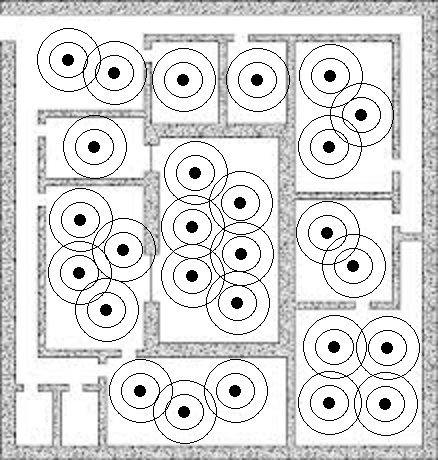
\includegraphics[width=5cm]{images/sensors.jpg}
    \end{figure}
  \end{columns}
\end{frame}

\begin{frame}
  \frametitle{Раскраска графа}
  \begin{columns}[c]
    \column{.5\textwidth}

    Условия:
    \begin{itemize}
      \item каждая вершина может быть раскрашена в один из трех цветов;
      \item смежные вершины должны быть раскрашены в разные цвета.
    \end{itemize}

    Обе задачи являются примером задачи с ограничениями.

    \column{.5\textwidth}
    \begin{figure}
       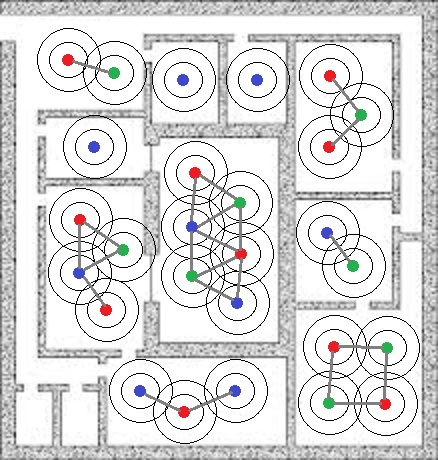
\includegraphics[width=5cm]{images/graph-coloring.jpg}
    \end{figure}
  \end{columns}
\end{frame}

\begin{frame}
  \frametitle{Задачи с ограничениями}
  Задача ограничениями:
  \begin{itemize}
    \item<1-> множество переменных (сенсор, вершина);
    \item<2-> множества возможных значений для каждой переменной (частота, цвет);
    \item<3-> множество ограничений (пересекающиеся сенсоры, смежные вершины);
    \item<4-> необходимо назначить каждой переменной значение, чтобы ограничения были выполнены.
  \end{itemize}
\end{frame}

\begin{frame}
  \frametitle{Задачи оптимизации}
  Задача \alert{оптимизации}:
  \begin{itemize}
    \item<1-> множество переменных (сенсор, вершина);
    \item<1-> множества возможных значений для каждой переменной (частота, цвет);
    \item<1-> множество ограничений (пересекающиеся сенсоры, смежные вершины);
    \item<2-| alert@2> функция веса для каждого нарушенного ограничения;
    \item<3-| alert@3> необходимо минимизировать сумму весов нарушенных ограничений;
  \end{itemize}
  \visible<4->{\alert{Задачи с ограничениями в общем случае NP-полные!}}
\end{frame}

\begin{frame}
  \frametitle{Распределенные задачи с ограничениями}
  В распределенной задаче оптимизации/с ограничениями переменные распределены между агентами.

  Обычно каждый агент отвечает за одну переменную.

  Задачи ИИ часто формулируются в виде задач с ограничениями.
\end{frame}

\begin{frame}
  \frametitle{Подходы к решению}

  Подходы к решению:
  \begin{itemize}
    \item адаптация классических решений \\ (перебор, нахождение решения во всём пространстве поиска);
    \item адаптация алгоритмов локального поиска \\ (нахождение оптимального решения в локальной области пространства поиска);
    \item кооперативные подходы \\ (в основном заимствованные из природы/социологии).
  \end{itemize}
\end{frame}

\begin{frame}
  \frametitle{Асинхронный перебор: основные концепции}
  \begin{figure}
    \includegraphics[width=11cm]<+>{images/ABT/concepts01.png}
    \includegraphics[width=11cm]<+>{images/ABT/concepts02.png}
    \includegraphics[width=11cm]<+>{images/ABT/concepts03.png}
    \includegraphics[width=11cm]<+>{images/ABT/concepts04.png}
    \includegraphics[width=11cm]<+>{images/ABT/concepts05.png}
    \includegraphics[width=11cm]<+>{images/ABT/concepts06.png}
    \includegraphics[width=11cm]<+>{images/ABT/concepts07.png}
  \end{figure}
\end{frame}

\begin{frame}
  \frametitle{Асинхронный перебор: разрешение конфликтов}
  \begin{figure}
    \includegraphics[width=11cm]<+>{images/ABT/concepts08.png}
    \includegraphics[width=11cm]<+>{images/ABT/concepts09.png}
  \end{figure}
\end{frame}

\begin{frame}
  \frametitle{Асинхронный перебор: алгоритм}
  \begin{figure}
    \includegraphics[width=11cm]<+>{images/ABT/algo01.png}
    \includegraphics[width=11cm]<+>{images/ABT/algo02.png}
    \includegraphics[width=11cm]<+>{images/ABT/algo03.png}
    \includegraphics[width=11cm]<+>{images/ABT/algo04.png}
    \includegraphics[width=11cm]<+>{images/ABT/algo05.png}
    \includegraphics[width=11cm]<+>{images/ABT/algo06.png}
  \end{figure}
\end{frame}

\begin{frame}
  \frametitle{Асинхронный перебор: раскраска графа}
  \begin{figure}
    \includegraphics[width=10cm]<+>{images/ABT/gc01.png}
    \includegraphics[width=10cm]<+>{images/ABT/gc02.png}
    \includegraphics[width=10cm]<+>{images/ABT/gc03.png}
    \includegraphics[width=10cm]<+>{images/ABT/gc04.png}
    \includegraphics[width=10cm]<+>{images/ABT/gc05.png}
    \includegraphics[width=10cm]<+>{images/ABT/gc06.png}
    \includegraphics[width=10cm]<+>{images/ABT/gc07.png}
    \includegraphics[width=10cm]<+>{images/ABT/gc08.png}
    \includegraphics[width=10cm]<+>{images/ABT/gc09.png}
  \end{figure}
\end{frame}

\begin{frame}
  \frametitle{Асинхронный перебор: итоги}
  Каждый агент отвечает за одну переменную и предлагает другим агентам принять значение,
  которое он выбрал.
  \begin{itemize}
    \item асинхронный перебор \cite{Bessiere2005} ~--- полный алгоритм;
    \item глобальное упорядочивание агентов;
    \item нет процедуры останова (но она легко добавляется);
    \item хорошо масштабируется.
  \end{itemize}

  Расширения:
  \begin{itemize}
    \item изменение порядка при конфликтах (AWCS \cite{Yokoo1995});
    \item решение задачи оптимизации (ADOPT \cite{Modi2003}, APO \cite{Mailler2006});
    \item динамическое добавление агентов (DynAPO).
  \end{itemize}
\end{frame}

\begin{frame}
  \frametitle{Другой подход: \\ распределенный локальный поиск}
  Алгоритмы распределенного локального поиска исследуют возможные изменения состояния:
  \begin{itemize}
    \item всегда стремятся улучшить состояние (уменьшить количество конфликтов);
    \item естественным образом поддерживают динамику (добавление ограничений, агентов);
    \item эффективны по времени;
    \item не полны и требуют настройки параметров.
  \end{itemize}

  Известные алгоритмы:
  \begin{itemize}
    \item Tabu search \cite{Glover1997};
    \item Simulated annealing \cite{Radenski2012};
    \item Iterative Breakout method \cite{Hirayama2005}.
  \end{itemize}
\end{frame}

\begin{frame}
  \frametitle{Другой подход: \\ кооперативные алгоритмы}
  Популяция ~--- это набор индивидуальных агентов.
  \begin{itemize}
    \item агент знает целиком исходную задачу (и может решить сам);
    \item агенты координируются для нахождения решения.
  \end{itemize}

  Известные алгоритмы:
  \begin{itemize}
    \item эволюционные и генетические алгоритмы \cite{Dozier2007, Handa2003};
    \item Particle Swarm Optimization \cite{Parsopoulos2002};
    \item Ant Colony Optimization \cite{Dorigo02}.
  \end{itemize}
\end{frame}

\section{Автономность в МАС}

\begin{frame}
  \frametitle{Мотивирующий пример: \\ устранение ЧС}
  Пример: авария с возгоранием в туннеле. Вовлечены несколько организаций:
  \begin{itemize}
    \item пожарная бригада;
    \item скорая помощь;
    \item полиция;
    \item администрация;
    \item участники происшествия:
      \begin{itemize}
        \item возможные жертвы;
        \item наблюдатели;
        \item участники дорожного движения.
      \end{itemize}
  \end{itemize}

  Все участники имеют общую цель: устранение ЧС. Обмен информацией важен для корректной
  координации и технологии играют существенную роль.

  При обсуждении проблем координации используется понятие автономности.
\end{frame}

\begin{frame}
  \frametitle{Автономность: определение}
  Как и для агента, не существует общепризанного определения автономности:
  \begin{itemize}
    \item автономность~--- ключевая особенность агентов;
    \item в переводе с греческого означает <<возможность самоуправления>>.
  \end{itemize}

  В многоагентных системах:
  \begin{itemize}
    \item агент должен проявлять социальную активность и учитывать других участников;
    \item агент должен быть отвественен за свои действия;
    \item баланс между этими требованиями приводит к появлению ``уровней автономности''
      и контролируемой автономности.
  \end{itemize}
\end{frame}

\begin{frame}
  \frametitle{Контролируемая автономность}
  \begin{exampleblock}{}
    {\large ``{\it Контролируемая автономность} ~--- это способность динамически
    обрабатывать внешние воздействия с учётом внутренних мотиваций.''}
    \vskip5mm
    \hspace*\fill{\small--- Bob van der Vecht \cite{Vecht2009}}
  \end{exampleblock}

  Контролируемая автономность означает способность агентов изменять
  уровень своей (или чужой) автономности:
  \begin{itemize}
    \item это одно из основных средств самоорганизации системы;
    \item делает прозрачным создание адаптивных систем;
  \end{itemize}
\end{frame}

\begin{frame}
  \frametitle{Уровни абстракции при принятии решений}
  Автономность рассматривается в контексте взаимодействия с другими агентами \cite{Falcone2001}
  (старшие агенты~--- на более высоком уровне абстракции, делегаты~--- на более низком):
  \begin{itemize}
    \item уровень автономности определяет, за какие решения отвечает делегат, а за какие ~--- старший агент;
    \item уровни автономности:
      \begin{itemize}
        \item исполнительный \\ (каким образом выполнить задачу);
        \item планирующий \\ (планирование задач для достижения цели);
        \item целевой \\ (создание и изменение целей);
        \item моральный \\ (когда и как менять уровень автономности) \cite{Verhagen2000}.
      \end{itemize}
  \end{itemize}
\end{frame}

\begin{frame}
  \frametitle{Социальная автономность}
  Агент может принимать или отказываться от порученных заданий \cite{Falcone2001}:
  \begin{itemize}
    \item чем менее специфицированную задачу может принять агент, тем выше его уровень автономности;
    \item изменение автономности ~--- изменение зависимостей от других агентов;
    \item причины для смены уровня автономности:
      \begin{itemize}
        \item агент не уверен, что может справиться с задачей;
        \item агент предвидит проблемы, которые могут возникнуть;
        \item агент считает, что может лучше справляться с большей автономностью;
        \item агент хочет ``удивить'' старшего сверхурочной работой.
      \end{itemize}
  \end{itemize}
\end{frame}

\begin{frame}
  \frametitle{Возможность и разрешения к действию}
  Автономность определяется свободой выбора и исполнения действий \cite{Bradshaw2004}.
  \begin{itemize}
    \item два аспекта: {\bf возможность выполнить} действие и {\bf разрешение на выбор} действия;
    \item действия различаются на
      \begin{itemize}
        \item потенциальные (возможные в данной среде);
        \item практически возможные (в текущем состоянии мира);
        \item возможные (для данного агента)
        \item если возможные действия агента совпадают с ``практически возможными'',
          он считается полностью автономным (по первому аспекту).
      \end{itemize}
  \end{itemize}
\end{frame}

\begin{frame}
  \frametitle{Влияние на групповые решения}
  Автономность измеряется вкладом в групповое решение \cite{Martin2006}:
  \begin{itemize}
    \item автономность агента определяется для каждого задания;
    \item в отношении задания у некоторых агентов может быть
      приоритет в плане принятия решения;
    \item уровень автономности определяется степенью независимости
      решения агента от решения любого другого агента.
  \end{itemize}

  Пример: агенты должны решить, в каком порядке они будут эксклюзивно
  пользоваться общим ресурсом.
\end{frame}

\begin{frame}
  \frametitle{Управление процессом принятия решения}
  Агент может передавать управление процессом принятия решения \cite{Scerri2004} другому агенту или человеку.
  \begin{itemize}
    \item агенты распологают набором стратегий для передачи управления;
    \item агенты могут менять ограничения (например,
      требовать дополнительное время на принятие решения);
    \item временные рамки определяют моменты передачи управления.
  \end{itemize}
\end{frame}

\begin{frame}
  \frametitle{Осознание автономности}
  Важной проблемой является осознание агентом своей автономности:
  \begin{itemize}
    \item осведомлённость о собственной автономности определяет основу ответственности;
    \item предполагается, что агент действует рационально и осознает свой выбор
      с учётом моральных законов;
    \item агент должен осознавать последствия принимаемых решений.
  \end{itemize}

  Агент, осознающий свою автономность не просто переключается между ``режимами'' работы,
  но оценивает последствия того или иного решения.
\end{frame}

\begin{frame}
  \frametitle{Регулирование воздушного траффика}
  Проблемы:
  \begin{itemize}
    \item пилоты коммерческих рейсов вынуждены полагаться на авиадиспетчеров;
    \item чтобы авиадиспетчеры могли справляться со своей задачей, в воздушном
      пространстве ``вычерчиваются'' специальные магистрали;
    \item самолёты регулярно стоят в очередях на такую магистраль;
    \item самолёты на магистрали должны поддерживать установленную скорость,
      чтобы избежать задержек;
    \item со временем растёт потребность в воздушном транспорте и, соответственно,
      увеличиваются задержки.
  \end{itemize}
\end{frame}

\begin{frame}
  \frametitle{Моделирование управления воздушным траффиком}
  Совместное управление воздушным траффиком:
  \begin{itemize}
    \item моделирование воздушного траффика;
    \item агенты ~--- диспетчерские центры (центральный, региональные и каждой авиалинии);
    \item цель ~--- максимально эффективно использовать магистрали;
    \item уровни автономности напрямую связаны с иерархией диспетчерских;
    \item в рамках одного уровня иерархии (одной компании) приоритеты могут меняться;
    \item контроль автономности производится людьми.
  \end{itemize}
\end{frame}

\section{Разработка многоагентных систем}

\begin{frame}
  \frametitle{Архитектура агента}
  Основные архитектуры агентов:
  \begin{itemize}
    \item {\it рассуждающие агенты} используют символьные вычисления
      и логический вывод для решения задач. Основные проблемы:
      \begin{itemize}
        \item представление задачи в логической системе;
        \item эффективная реализация процесса вывода.
      \end{itemize}
    \item {\it реактивные агенты} используют набор поведений для
      эффективной работы в реальном мире. Полагается на эвристические
      алгоритмы.
    \item {\it гибридные архитектуры} объединяют преимущества обоих подходов.
  \end{itemize}
\end{frame}

\begin{frame}
  \frametitle{Структуры многоагентной системы}
  При создании структуры МАС используются:
  \begin{itemize}
    \item {\it организационные шаблоны} \\
      (формирование известных соцальных структур);
    \item {\it фрактальные системы} \\
      (агенты объединяются в группы, которые действуют как единый агент);
    \item {\it поведенческие паразиты} \\
      (среда воздействует на внутреннее состояние агента, имитируя симбиоз).
  \end{itemize}
\end{frame}

\begin{frame}
  \frametitle{Средства разработки МАС}
  Существует множество средств разработки МАС. Из них стоит выделить
  3APL, Jason, Jack, IMPACT, JADE, Jadex, DEFACTO, ARTIMIS.

  Большинство общих фреймворков нацелено на использование ментальных
  характеристик агента. Они предоставляют возможность задания целей
  агента при помощи специальных языков вроде AgentSpeak \cite{Rao1996}.

  Некоторые среды позволяют упростить программирование процесса принятия
  группового решения.

  К сожалению, ни одна среда не предоставляет библиотеки
  распределенных алгоритмов, структурных или архитектурных шаблонов.
\end{frame}

\begin{frame}{}
\addtocounter{framenumber}{-1}
\begin{center}
\LARGE{Спасибо за внимание!}
\end{center}
\end{frame}

\section{Список литературы}

\begin{frame}[allowframebreaks]
  \frametitle{Список использованной литературы}
  \bibliographystyle{alpha}
  \bibliography{agent-slides}
\end{frame}

\end{document}

